


\chapter{Implementation}
This chapter discussed the technical implementation of the system based on the design discussed before. Section 3.4.1 provide the technical information about the main entity as classes that will be used in this study, including its properties and methods.
section 3.4.1 to 3.4.5 provides Information about the class activities of the application.Section XX provides an information about the notification. Lastly, section XX provides an information about the tracker.

\todo{put the chapter number}

Flask framework and python programming language is used to develop the webserver. Java programming language and Android SDK is used to develop android application.

% \subsection{Web server}
% explain sending data to the android application
% Webserver is a http server that
% send a json file


%explain get data from android appplication


\section{Entities relationship}
All the entities discussed on the design chapter will be represented as a class which consist of variables and methods.
The relationship between classes can be seen on the class diagram on figure \ref{fig:class_diagram}.
 The box present the class. The upper part of the box consist of the variable name and its type.
 The plus and minus sign before the variable name present the scope of the variable.
  Minus (-) means private and plus (+) means public.
  The bottom part of the box consist of the class methods and the type of it's output.
  Furthermore, The arrow present the variable relationship whether it can be one-to-one (1..1)  or one-to-many(1..*) relationship.
  It also present the class extend other class (it has same properties and methods).

\begin{sidewaysfigure}[ht]
\begin{center}
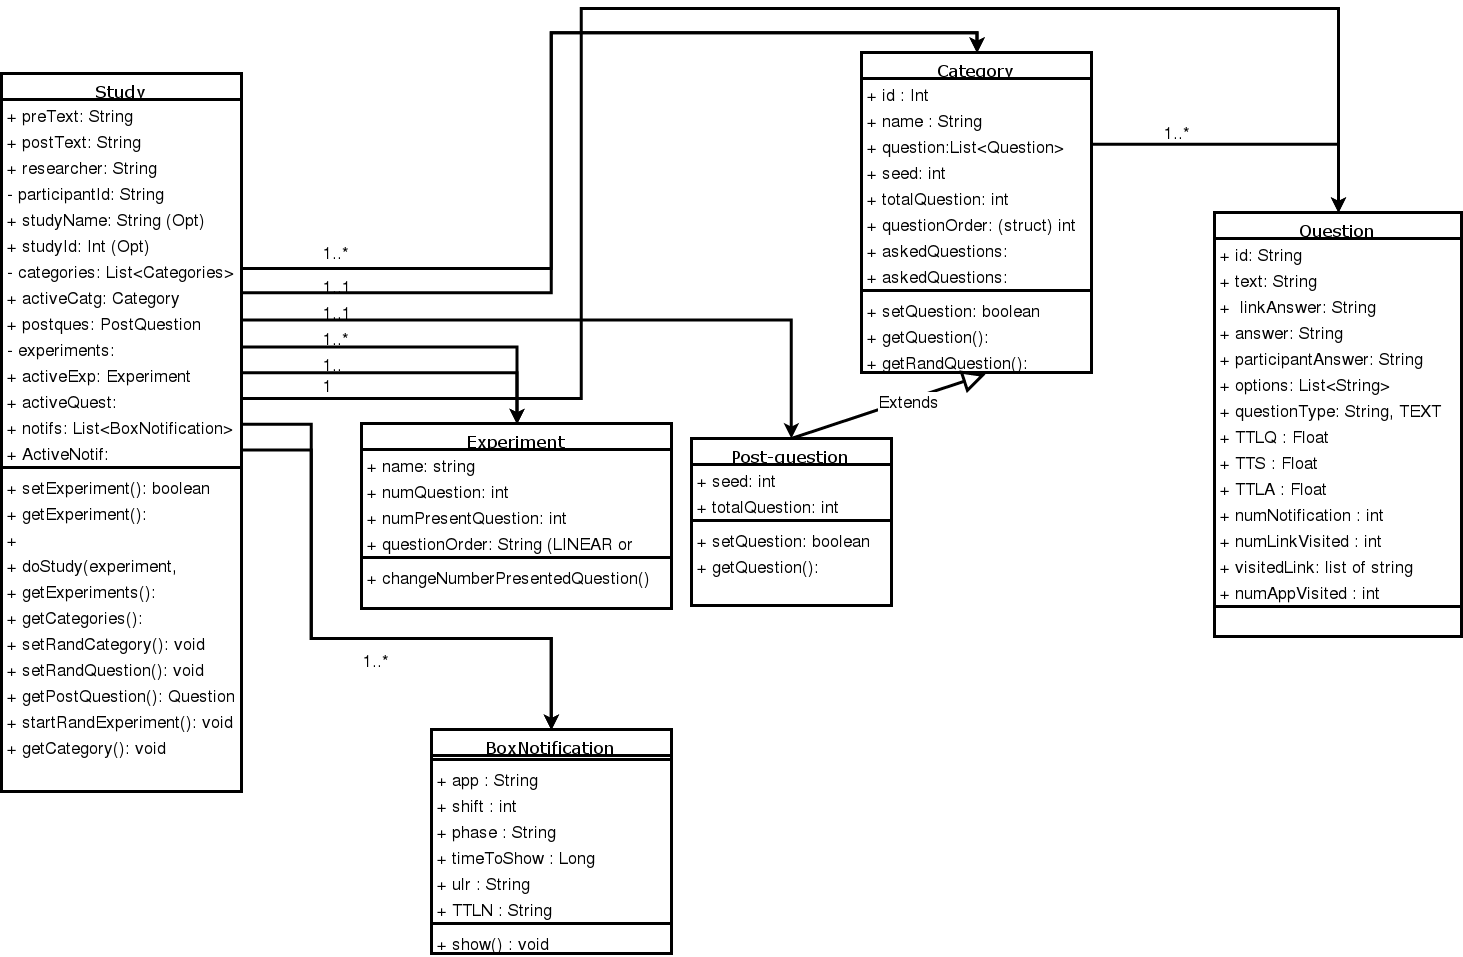
\includegraphics[scale=0.3]{class_diagram}
\end{center}
\caption{Class diagram of the application}
\label{fig:class_diagram}
\end{sidewaysfigure}

\subsection{Study Class}
Study class is the class that act as a main container for other entities of the application, and it control the flow of the main function of the experiment.
Some of its properties are defined from input file; \textit{preText, postText, researcher, studyName, studyId}.
As seen in the class diagram \ref{fig:class_diagram}. The study class contains \textit{experiments} variable which consist of list of experiment objects.
 \textit{Categories} variable which consist of list of category objects, and \textit{notifs} variable that consist of list of notification objects.

As explained in the design section,
the experiment application need to initialize following variables before conducting the experiment;
\textit{ActiveExp} (active experiment) variable is experiment that will be conducted, and \textit{activeCatg} (active category) is the
category that will be used to pick questions.
\textit{ActiveQuest} (active question) variable present what questions are currently asked to the participant.
The question inside \textit{activeQuest} variable are picked from the list of questions inside the active category (\textit{activeCatg}) variable.

\textit{ActiveExp} is set by the researcher on the setting experiment window, \todo[inline]{refer to appendix}.
the \textit{activeCatg} is chosen by the participant during the experiment, refer to an appendix.



%After the category (\textit{activeCatg}) and set the experiment %(\textit{activeExp}) are chosen, the experiment can be started. The experiment will present the participant with one or several questions. In the study class there is \textit{activeQuest} (active question) variable that contains the  question objects that is being on a \textit{shift}.

Moreover, the class also contains \textit{activeNotif} (active notification) variable.
This variable contains a list of notifications that has been presented to the participant.
The notification object is picked from the \textit{notifications} variable that contains all the notification.

% \begin{table}[!b]
%   \centering
%   \begin{longtable}{ |p{0.5cm}|p{4cm}|p{2.3cm}|p{6cm}|  }
%  \hline
%  No& Variable's name & Type & Description \\
%  \hline
%  1 & preText & string  & the text\\
%  2 & postText & string & THIS DESCRIPTION NEED TO BE FILLED\\
%  3 & researcher & string & True if the participant decide to look at the question again, false otherwise. \\
%  4 & studyName & string & total time (in millisecond) when the participant see the answer links and decide to look the question again or answer the question (next button) \\
%  5 & studyId & string & Similar with TTLB and the participant decide to look at the question again.Then, answer links are shown again to the participant\\
%  6 & participantId & List of String & The list of links clicked/visited by the participant after clicking the answer links\\
%  7 & randomGenerator & List of Long  & List of the total time (in millisecond) the participant stay on a page after clicking link\\
%  8 & categories & List of String & similar with visited\_links but the participant have decided to see the question again then return to the answer links window\\
%  9 & experiments & List of Long & Similar with time\_visited\_links but the participant decide to look at the question again then click the answer links\\
%  10 & postques & Long & Total time (in millisecond) the participant see the fill answer window and then click next\\
%  11 & activeExp & Long & Total time (in milisecond) the participant write the answer on the text box\\
%  12 &  activeCatg & Integer & how many notification is shown during the a question \\
%  14 & activeQuest & Long & Total time (in millisecond) it tooks the participant after clicking the notification to back to experiment application\\
%  15 & notifs & Long & Total time (in millisecond) it tooks the participant after clicking the notification to back to experiment application\\
%  16 & activeNotif & Long & Total time (in millisecond) it tooks the participant after clicking the notification to back to experiment application\\
%  16 & shiftNum & Long & Total time (in millisecond) it tooks the participant after clicking the notification to back to experiment application\\

% \hline
% \end{longtable}
% \caption{Variable inside study class}
%  \label{tab:studyClassVariable}
% \end{table} \par
\subsection{Experiment Class}
The Experiment class contains the \textit{experiment variables} that is used to define the behavior of the experiment. The variables is explained in the table \ref{tab:ExperimentClassVariable}.
Every variables inside this class except \textit{numPresentedQuestion} is determined from the input file. \textit{numPresentedQuestion} is a variable that
control how many questions is presented to the participant each time.
 \textbf{changeNumberPresentedQuestion()} method is called by the study class to change the value \textit{numPresentedQuestion} variable.
 The change can be random (from 1 to \textit{maxPresentedQuestion}) by using using the Random object (RandomGenerator)
  provided by Java API.

\begin{table}[!htb]
  \centering
  \small
  \footnotesize
\begin{tabu}{|X[0.5,l]|X[5,l]   |X[2.3,l]|X[6,l]|  }
 \hline
 No & Variable's name & Type & Description \\
 \hline
 1 & name & string  & The name of the experiment\\ \hline
 2 & numQuestion & Integer & The number of questions will be asked on the experiment \\ \hline
 3 & numPresentedQuestion & Integer & The number of question presented to the participant on the experiment every phase of question-answer \\ \hline
 4 & questionOrder & String & If the value is RANDOM, then the question is picked randomly from a list of question, if the value is LINEAR then the question will be picked based on the order of the input file \\ \hline
 5 & randomPresentedQuestion & Boolean & If it the value is true, then on each phase the num of presented question will changed randomly, explained more on changeNumberPresentedQuestion method \\ \hline
 6 & maxPresentedQuestion & Integer & This is the maximum number of presented question if the number of presented question is decided randomly\\ \hline
 7 & randomGenerator & Random  & This is a random class that use to generate random nunmber, it is used inside changeNumberPresentedQuestion method \\ \hline
\end{tabu} \par
\caption{variables inside the experiment class}
 \label{tab:ExperimentClassVariable}
\end{table}

\subsection{Category Class}
Category class is used to carry the questions objects.
It has two main variables; \textit{questions} and \textit{askedQuestion}.
\textit{Questions} variable consist a list of questions. This variable is filled by
the question from the input file.
\textit{AskedQuestion} variable consist of all the question that had been asked.

The class has two main methods \textit{getRandQuestion()} and \textit{getQuestion()}.
These methods will be called during the quiz activity to put question object into activeQuestion variable.
These method are two different procedure to pick a question from \textit{questions} variable.
the former take the question randomly while the latter take the question based on the order of the input file.
Java random class is used to generate random index (from 0 to the size of the \textit{questions} variable).
After the question is selected, it will get deleted from the \textit{questions} variable and then it will be put it into \textit{askedQuestion} variable.

\subsection{Question Class}
Table \ref{tab:questionClassVariable} shows the variables inside this class.
The Question class consist of the content of question; it's question text, answer link and answer.
The class is also contains the tracked variable (the variables is explained more on trackker section).
The question can be two type MC or TEXT. MC means multiple choice, this question type will have multiple options on it's answer,
and the participant can chose one of them. while TEXT means that the participant need to write the question.
\textit{representId} generate when the questions are presented to the participant. this variable is unique and can
be used to classify which questions are presented at the same time.

\begin{table}[!tbh]
  \centering
  \small
  \footnotesize
  \begin{tabu}{|X[0.5,l]|X[4,l]|X[2.3,l]|X[6,l] |}
 \hline
 No & Variable's name & Type & Description \\
 \hline
 1 & id & string  & The id of the question.\\  \hline
 2 & text & string & The text of the question.\\ \hline
 3 & linkAnswer & string & the URL link to the answer page. \\ \hline
 4 & answer & string & (optional) the answer of the question. \\ \hline
 5 & participantAnswer & string & the answer of the participant during the quiz activity.\\ \hline
 6 & questionType & String & The type of the question. The value can be "MC" or "TEXT".\\ \hline
 7 & representId & string  &  the random id generated when the question is presented during quiz.\\ \hline
 7 & options & list of String  & The answer option if the question is multiple choice.\\ \hline
\end{tabu}
\caption{Variable inside Question class (without the tracked variable)}
 \label{tab:questionClassVariable}
\end{table} \par

\subsection{BoxNotification class}
BoxNotification is used as a class name because the name Notification is already defined inside the Android framework.
Most of the variable in this class is similar on the defined variable on the design section.
Similar to the question class, the notification also contain \textit{presentedID} which show
on which question the notification is popped up.
The content of the notification can be set into \textit{title} and \textit{msgText} variable.
The Notification can open an android application of twitter, facebook, instagram and web browser. The application should be installed to the phone, otherwise the notification will open the url of the application on the web browser.
To define which user will be shown if the user clicked the instagram, twitter or facebook notification. The user
is defined by the user\_id code which can be found on the profile of their social media.
the url can also contains the URL link, then the application will open the web page.
This app need to be specified on the \textit{app} variable and the \textit{url} variable. The \textit{url} variable need to be filled with the user id of the twitter or instagram. Or it can be filled with http/https url to open web page. the class contains a show() method that will pop up the notification in the android phone.
The the mechanism and flow of the notification will be explained on next chapter.

%
% \begin{table}
%   \centering
%   \small
%   \footnotesize
% \begin{tabu}{ |X[0.5,l]|X[4,l]|X[2.3,l]|X[6,l]|  }
%  \hline
%  No& Variable's name & Type & Description \\
%  \hline
%  1 & url & String & this contains  \ \hline
%  2 & titleText & Integer & this is the maximum number of presented question if the number of presented question is decided randomly\\ \hline
%  3 & msgText & Random  & this is a random class that use to generate random nunmber, it is used inside changeNumberPresentedQuestion method \\ \hline
%  4 & presentedID & Random  & this is a random class that use to generate random nunmber, it is used inside changeNumberPresentedQuestion method\\
% \hline
% \end{tabu}
% \caption{variable inside notification class, some of the variable are already discussed on the design section}
%  \label{tab:NotificationVariable}
% \end{table}

\section{Application flow}
In this section the flow of the application from the technical point of view is provided.
The flow of the application can be seen
on the figure \ref{fig:flowOfApplication}. The figure shows the flow of the application after input file is uploaded and
the experiment just have started.
As it seen in the figure, the flow is divided into four scope;
\begin{itemize}
\item \textbf{Setting}  : the researcher can set some properties of the experiment or choose to start the experiment.
\item \textbf{Experiment} : The participant conduct the quiz experiment.
\item \textbf{Notification} : The notification can be popped up during the quiz.
\item \textbf{PostQuestion} : The participant presented with post questions.
\end{itemize}
\par

To have further understanding about the application flow, the activitues and method on the flow chart is explained further on the following subsection.



\begin{figure}
\begin{center}
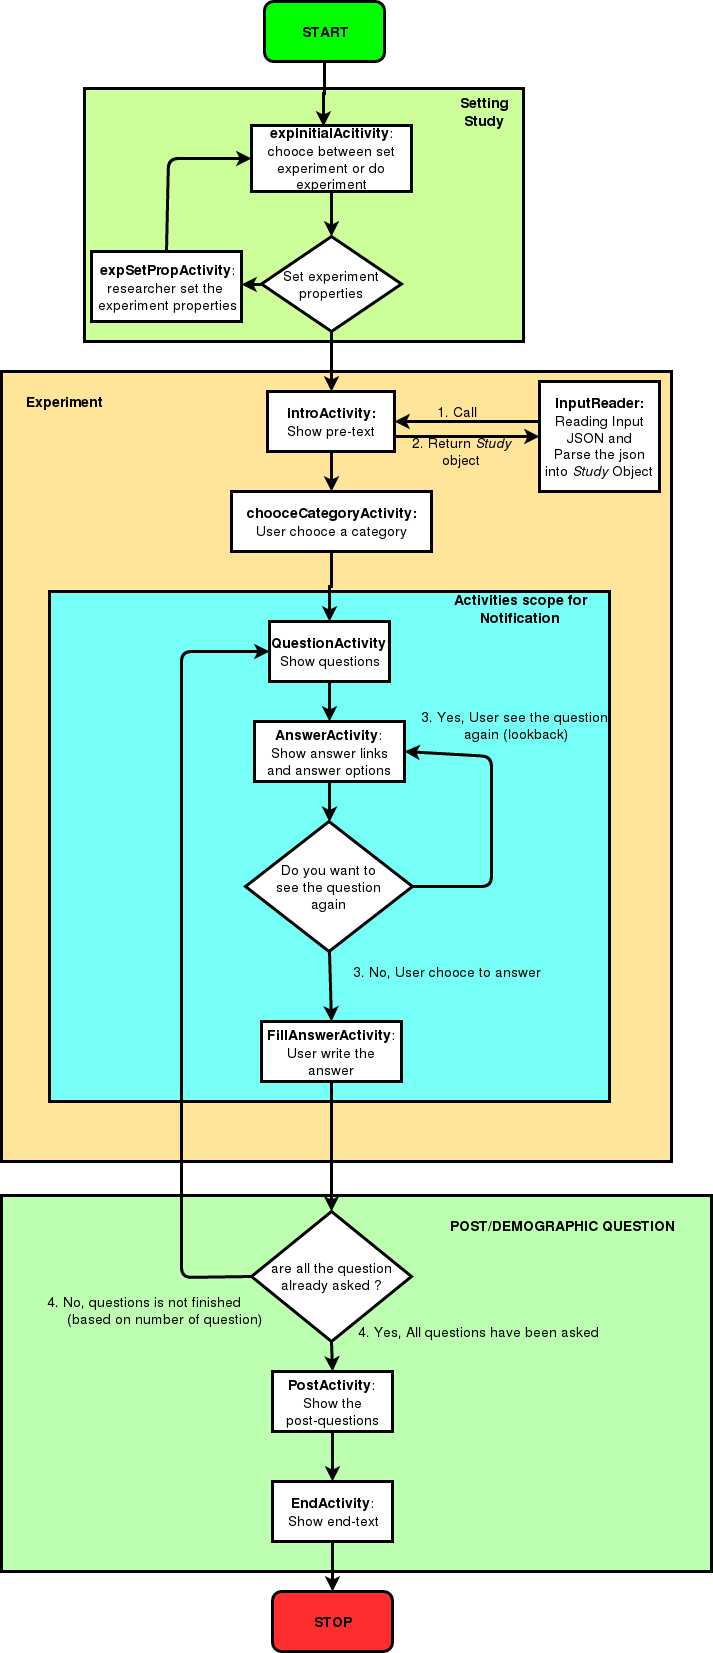
\includegraphics[scale=0.4]{Flowchart_}
\end{center}
\centering
\captionsetup{justification=centering}
\caption{The flow of the application}
\label{fig:flowOfApplication}
\end{figure}

\subsection{Android Activity}
The android application built upon multiple class activities.
Each activities has an user Interface (UI) template. this template is saved into a xml file. The template consist of UI element, for example button, text, etc.
Its corresponding class activity will decide what will appeared on the phone or what happen if a button is clicked.
For example answerActivity class will have activity\_answer.xml template.
The activity class is used to catch the event such us clicked or move to another application. these event is linked to an \textit{event listener} methods.

The android application also contains a lifecycle which is  default methods and activities that will be called every time.
Figure \ref{fig:theLifeCycleOfActivity} shows the android activity lifecycle \citep{androidActivity}.
There are three methodes inside the lifecycle that is used in this experiment application;
 \textit{OnCreate()} is the first method to get called everytime the activity start.
 \textit{OnPause()} will be called if the user move / redirected to another application.
 Lastly,  \textit{OnResume()} is called if the user open the application again after leave the application.

\begin{figure}[!tbh]
\begin{center}
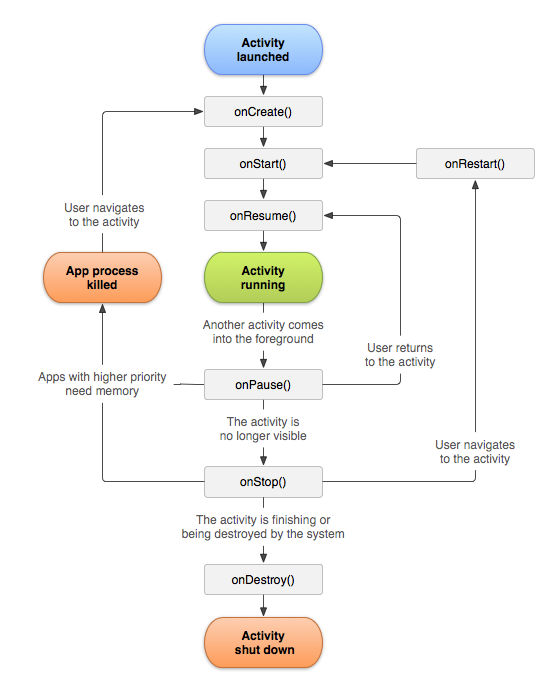
\includegraphics[scale=0.5]{activityLifeCycle}
\end{center}
\centering
\captionsetup{justification=centering}
\caption{The lifecycle of android application}
\label{fig:theLifeCycleOfActivity}
\end{figure}



\subsection{expInitialActivity}
The UI layout of these activity can be seen in figure \todo[inline]{refer to an appendix}.
The participant can click a button to begin the experiment or to set the properties of the experiment.
On the \textbf{OnCreate()} method the \textbf{InputReader.read()} method is called firstly.
This method will read the JSON input and compiled it into \textit{Study} object.
String input is compiled into json object by using \textit{GSON} library.
\textit{GSON} is a serialization / deserialization library that is used to convert string into json object or another way around. \citep{gsonLib}

Then the json object compiled into The \textit{Study} object. This object controlled the quiz experiment and hold all the data, including the track variables.
This object will be sent through the activites.
\textit{Intent} class of java is used to encapsulate the object and send to another activity.
Because the \textit{Study} object need to be encapsulated inside the Intent,
 java programming language require every class including the Study class to implement \textit{Serializable}.


\begin{figure*}
\centering
\begin{minipage}[b]{.4\textwidth}
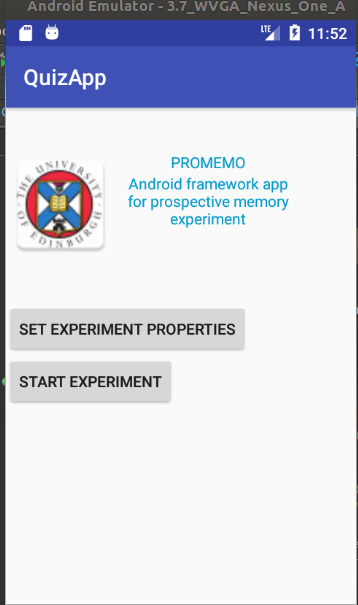
\includegraphics[scale=0.32]{FE_1}
\caption{Caption}\label{label-a}
\end{minipage}\qquad
\begin{minipage}[b]{.4\textwidth}
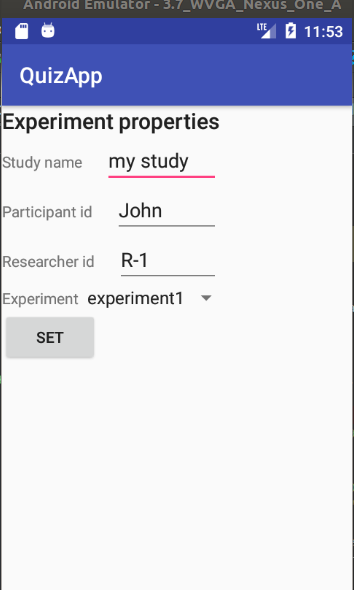
\includegraphics[scale=0.32]{FE_set_properties}
\caption{Caption}\label{label-b}
\end{minipage}
\end{figure*}

\subsection{expSetPropActivity}
This activity is used to set some parameter of the experiment. In this activity the researcher can pick which experiment to conduct, the name of the experiment,
the id of the researcher and the id of the participant.
The purpose of this activity is to make it easier for the researcher to conduct multiple experiment and multiple participants without uploading the input file again.
 Figure XX shows the layout of the activity
 \todo[inline]{attach appendix}

\subsection{IntroActivity}
This activity is used to show the information about the experiment to the participant before starting the experiment.
These information is obtained from the preText and postText variables. the value of this variable will be converted into html and shown to the participant.
Figure X show example of the Consent information shown inside the application.
\todo[inline]{attach appendix}

\subsection{ChooseCategoryActivity}
In this activity the participant choose which category he/she want to answer, as seen in the figure XX.
\todo[inline]{Also do I need to attach my code here?}
The selected category name will then save in the \textit{selectedCategoryName} variable inside study class.
\textit{selectedCategoryName} is used to in the experiment initialization to initialize \textit{activeCatg} variable


\subsection{QuestionActivity}

In this activity, the question inside activeQuestion variables are shown to the participant.
This activity will be called multiple time during the quiz experiment.
the activity mainly call \textbf{Study.runExperiment()} method on the \textbf{OnCreate()} event listener.
\textbf{Study.runExperiment()} is used to start or continue the quiz experiment. this method is explained on the section below.

\subsubsection{Study.RunExperiment()}
This method will be called everytime the Quiz activity started.
The main function of this methods are :
\begin{itemize}
\item Initialize the active experiment (\textit{activeExp} variable) and active category (\textit{activeCatg}) variable.
\item Change the number of \textit{presentedQuestion} (the variable is explained in the Experiment class section).
\item Set the active questions (\textit{activeQuest}) from the questions in the category.
\end{itemize}


\begin{figure}
\begin{center}
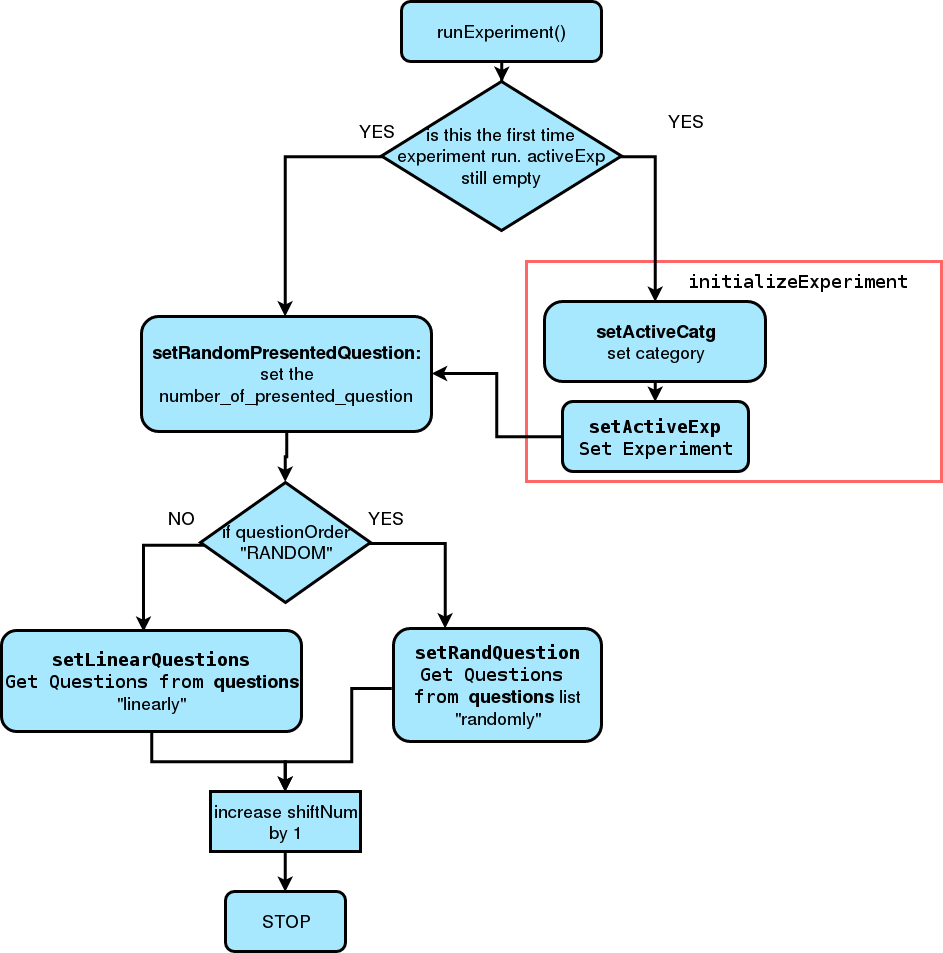
\includegraphics[scale=0.5]{runExperiment}
\end{center}
\caption{runExperiment flow chart}
\label{fig:runExperiment_flow}
\end{figure}


Figure \ref{fig:runExperiment_flow} shows the work flow of the method. The First step is to initialize the experiment by checking the active experiment (\textit{activeExp}) variable.
 if it's empty than it's mean that it's the begining of the experiment, hence some variables needs be initialized. If it's mean that the experiment had been started (on-going)
 so new question is presented to the participant.


On the intialization, active experiment (\textit{activeExp}) and active category (\textit{activeCatg}) are initialized by calling \textbf{initializeExperiment} method.
The \textbf{initializeExperiment} method will fetched the selected \textit{experiment} and the
\textit{category} object from the study class variables based on the \textit{selectedExperimentName} and \textit{selectedCategoryName}.


Subsequently, the \textbf{setRandomPresentedQuestion()} is called, this method will set the value of numPresentedQuestion.
If the researcher set randomPresentedQuestion to true in the input file, then \textbf{Experiment.changeNumberPresentedQuestion()} is called, this method will set numPresentedQuestion randomly
On the other hand if it's false, then the numPresentedQuestion will be constant.

Next, \textbf{isExperimentIsStillGoing()} is called. This method make sure if the experiment is still on progress by checking the size of the
\textit{question} variable inside the \textit{activeCatg}. If the size is still larger or similar than \textit{numPresentedQuestion} then the experiment can be continued.

Lastly, the active question (\textit{activeQuest}) is picked from the questions variable by calling \textbf{setActiveQuestion()}. this method filled
 i \textit{activeQuest} variable by fetching \textit{question} object from the \textit{question} variable inside \textit{activeCatg} object.
  The question object will be picked randomly if the researcher set \textit{questionOrder} to random. Otherwise, it will be picked linearly based on
  the input file order.


\subsubsection{AnswerActivity}
In this activity the answer link are shown as a textview inside the UI layout. If the participant click the answer
link then the \textbf{clickListener()} method inside the textview will open the answer page.
A java class called \textit{webview} is used as a browser. The \textit{webview} will open the web page based on the URL of the answer link (\textit{question.url}).

On the layout, two radio buttons are presented to the participant. These are the option whether the participant want to return to see the question again or to continue
 to answer the question.
If the participant chose to look at the question again then a speical string is capsulated inside the \textit{intent} object.
This string is sent to question activity then send back to answer activity. this string is used to indicate if the participant look at the question again.
If the string is sent to answerActivity then the radio button "to see the question again" is hidded by setting its visibility to GONE.
\todo[inline]{put the snapshot of the code}


\subsection{fillAnswerActivity}
In this activity the participant should answer the question by writing the answer on the editText UI as seen on figure XX.
\todo[inline]{Also need to include pics}

If the participant click next button then \textbf{saveAnswer()} method is called. this method will get the value of the editText
and stored it on the \textit{participantAnswer} variable inside the \textit{question} object.


\section{Notification mechanism}
Figure \ref{fig:NotificationFlo} shows the mechanism of notification.
As seen on the flowchart, the \textbf{Study.checkNotification()} method is called inside
the OnCreate event on the QuestionActivity, AnswerActivity and FillAnswerActivity.
The method check on every notifications inside the \textit{notifs} variable if the there is a notification that should be shown up based on \textit{phase} and \texit{shift} variable of the notifiaction.

If there  is a notification that need to be shown up then the notification object is added into the \textit{activeNotif} and it is deleted from the \textit{notifs} variable of the study object.

The notification need to wait for some millisecond before it can be shown up. The waiting time is defined in \textit{timeToshow} variable inside the BoxNotification class.
While the notification process wait, the main activity should keep working, so another process need to be spawned a part from the main process.
To accomplish it, \textit{TimerService} class is used. This class will be spawn as new process and it will sleep for \textit{timeToShow} millisecond.
After that, the service class will call the \textbf{BroadcastReceiver()}.
The \textbf{BroadcastReceiver()} method  is defined on all of activities, and it simply call \textbf{show()} method of the notification.
The \textbf{Notifaction.show()} method is used to show  the notification to the front end of the android screen. This methode use
 \textit{NotificationCompact.Builder} to build the notification layout.
 an \textit{Intent} object is inserted inside the Builder object that contains what application to open.
 If the participant click the notification then the experiment application will be minimized.
 This event will call \textbf{OnPause()} method on the current activity, and the android phone will open the intended application.
 The participant if the open the experiment application again, then the \textbf{OnResume()} method is called.


\section{Tracker}

The tracked variable are shown on the table \ref{tab:trackedVarible}.
All of these variable are stored inside the \textit{question} class as it seen in the class diagram \ref{fig:class_diagram}.
Some of the variables use to track the time in millisecond.
To track the time the \textit{stopWatch} class provided by java API is used.
The StopWatch object is stored inside the study class because the StopWatch class is not serizable which means
it can not be pass in the Intent object inside the Study class, so it is placed on the activity class.

During the experiment the application is minimized (participant click the notification).
Then event some Stopwatch object need to be pause. Inside \textbf{OnPause()} event listener the stopWatch is suspended,
and it will resume again inside the \textbf{OnResume()}.

As it seen in the class diagram, each one of tracked variable has it's own \textit{stopWatch} object for example \textit{stopWatchTTLQ} will track the time for TTLQ variable.
To stored the time tracked by the stopwatch the \textbf{study.log()} method is called.
this method pass two arguments, what variable to track and the stopwatch object used to track it.
for instance log("TTLQ",stopWatchTTLQ) will track the TTLQ variable and use stopWatchTTLQ to get the tracked time.
How each variable is tracked is explained further on the subsection below.

\subsubsection{TTLQ, lb\_TTLQ and lookback}
These variable is tracked inside the QuestionActivity.
StopWatchTTLQ and stopWatchTTLQ\_lb is used to track the timing of this variable.
The stopwatch object start to count the time when \textbf{OnCreate()} method is called on the current activity,
and the stopwatch will be stopped when the participant click next button. The \textbf{Study.log()} method will be called to track the variable when the next button is clicked.
 Inside the \textbf{Study.log()} method, it will call \textbf{logTTLQ()} methods to stored the value of the tracked variable on each question object inside the \textit{activeQuest}.
the stopwatch variable will be passed on these method and the milisecond didapat bycalling \textbf{StopWatch.getTime()} method.
The lookback variable will have true value if the participant chose to see the question again. These variable is set on the logTTLQ\_lb() method.

\subsection{TTLB and lb\_TTLB}
These variable are tracked inside the AnswerActivity. Similar with TTLQ,
stopwatchTTLB and stopWatchTTLB\_lb is used to track these variable.
The stopwatch will start on \textbf{Oncreate()} method and it will be tracked when the participant click the next button.

\subsection{visitedLinks, timeVisitedLink}
These variable is tracked inside the AnswerActivity.

During the AnswerActivity if the participant click the answer link then the \textit{webview} class of
java is used to open the URL link. StopWatchLink then will be started, and it is used to track the time participant have spent on each web page inside the webview.
The mechanism of the tracking is shown in the figure \ref{fig:webViewTrack}. Firstly, the prevUrl variable is initialized,
this variable stored the previous link the webview had opened. This webview class has an event listener called onPageFinished() which will called every time the web page
 has been finish loaded for example when the participant click the answer link or visit another link on the webpage. Every time the event listener onPageFinished() is called,
 or when the participant click the button then updateVisitedLinks() method is called. updateVisitedLinks() method stored the value of prevUrl (because it has been visited before)
 to visitedLinks variable and how long the participant spent on the web page to timeVisitedLinks.
\todo[inline]{check again}

\subsection{TTLA and TTLFA}
These variable are tracked on the fillAnswerActivty. the TTLA simply tracked similar to TTLQ and TTLB, the variable tracked using StopWatchTTLA.

TTLFA is tracked differently because if there is more than one question then there will be multiple editText for the answer field.

On each editText element, the event listener called OnFocusChangeListener is attached to it. this event listener will be called if the is a
change of focus on the UI layout of the activity, for example if the user click one editText then click another one. the event listener
 method can give an UI id of which editText was the user writing on before moving to another editText. the UI id will be stored inside the activeViewId variable.

{should I attach some code}. After getting the UI id a stopwatch corresponding on the editText should be obtained to track the time.
To accomplish this stopWatchTTLFA is made as a hashmap where the key is the UI id, the id is made from the index of the question inside the activeQuest variable,
and the value is the stopwatch correspond to the editText answer. so to access which Stopwach object correspond to particular editText the UI id from the event listener
will be used to get the corresponding stopwatch object.

to track the time updateTTLFA() method is called this method will track the TTLFA time by accessing the stopwatchTTLFA hash map using the activeViewId variable.


\subsection{numNotif, numNotifClicked and TTLN}
As explained on the section 4.3.8 during the QuestionActivity, AnswerActivity and fillAnswerActivity the checkNotifaction()
will find the notification that should be shown up to the screen and it will called the inceraseNumNotif() method.
This method will increase the numNotif variable of every question inside activeQuest.

If the notifaction is clicked then the inceraseNumNotifisClicked() method will be called inside the broadCastReceiver on the current activity class.
This method will increase the number of numNotifClicked variable on every question object inside the activeQuest variable.

notifStopWatch object is used to track the TTLN time. After the participant click the notification than the application will be minimized and other
application will be opened. As explained on the Android activity section (4.3.1), the OnPause() event handler will be called just before the application is minimized.
On OnPause() method a Study.startLogNotif() method is called, this method will start the notifStopWatch object.
Then after the participant got back to the experiment application the onResume() method is called. This method will call Study.stopLogNotif() method.
This method will get the current notification and set the TTLN from the notifStopWatch.
\cite{Kliegel1984}

%\todo[inline]{WHAT THE FUCK TO WRITE}

\begin{sidewaysfigure}[ht]
\begin{center}
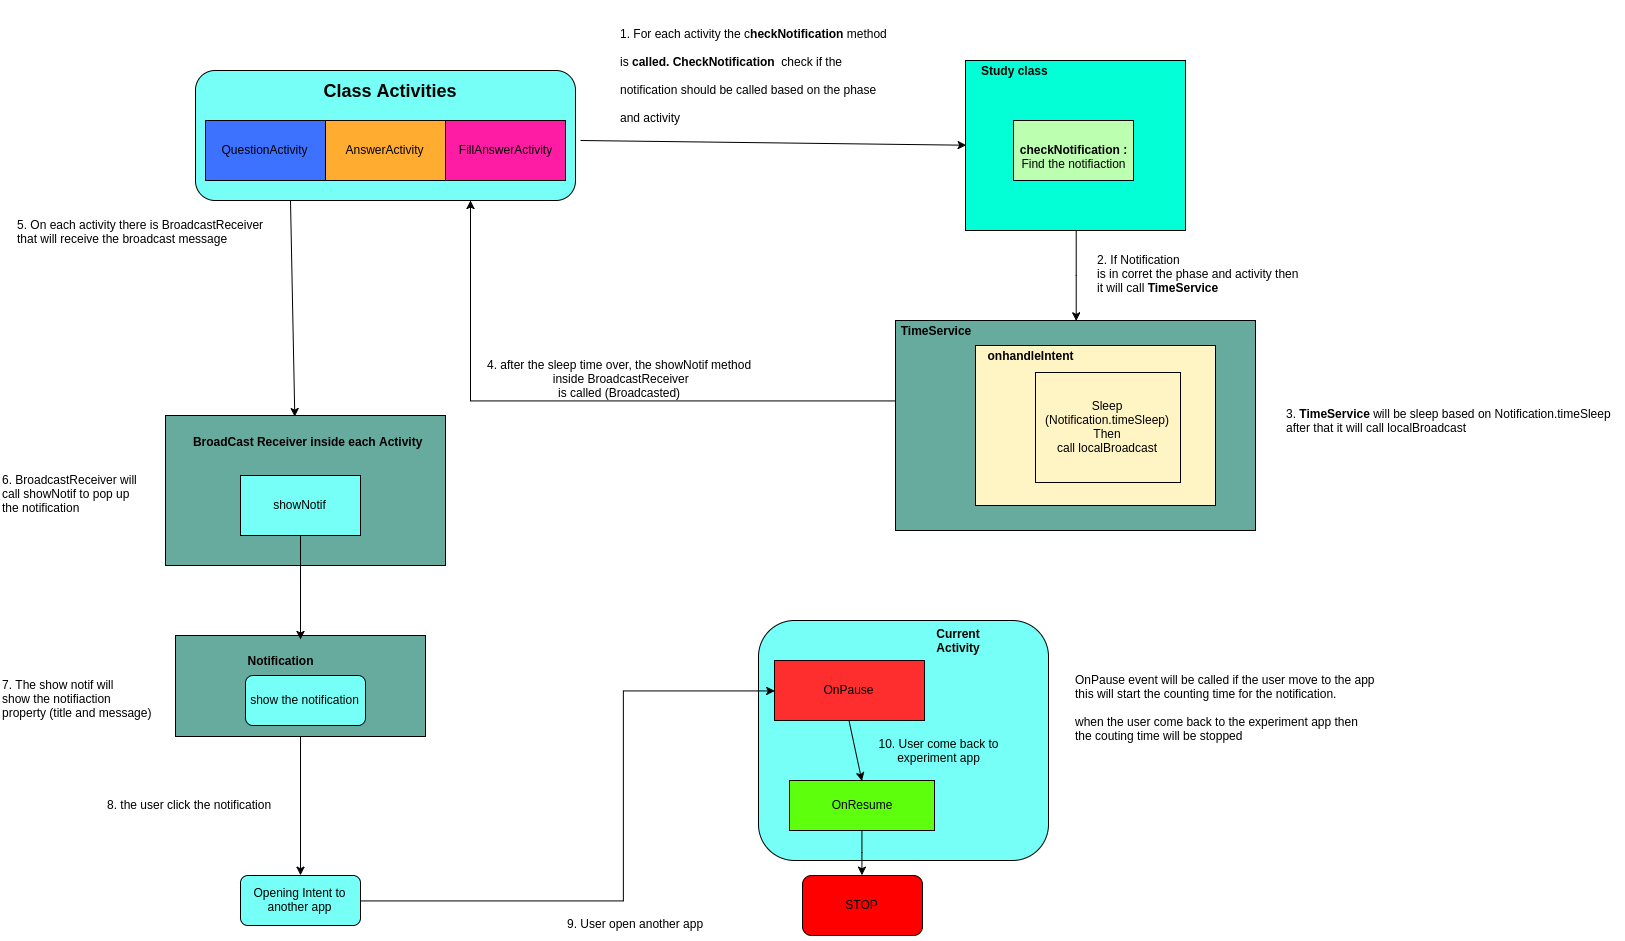
\includegraphics[scale=0.35]{notification_diagram}
\end{center}
\caption{The flow of the notification}
\label{fig:NotificationFlo}
\end{sidewaysfigure}

\begin{figure}
\begin{center}
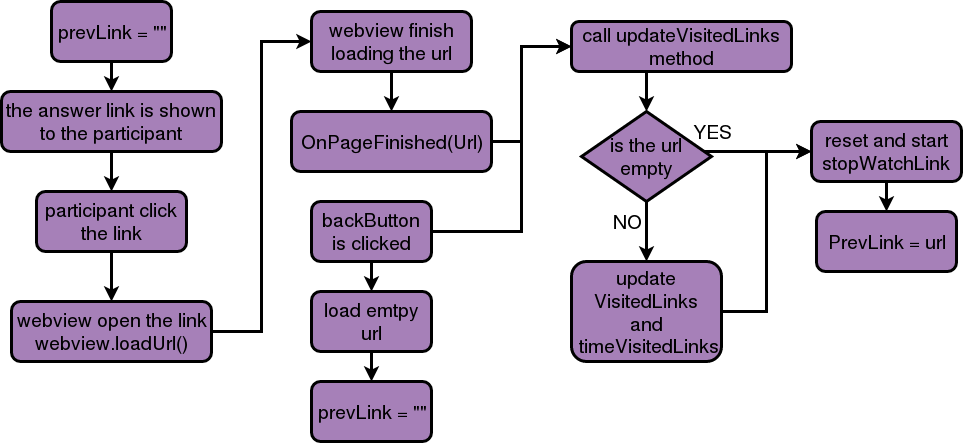
\includegraphics[scale=0.5]{tracker_linkVisited}
\end{center}
\caption{tracker mechanism for webview}
\label{fig:webViewTrack}
\end{figure}
